\documentclass[11pt,a4paper]{article}
\usepackage[utf8]{inputenc}
\usepackage[spanish]{babel}
\usepackage[IL2]{fontenc}
\usepackage{amsmath}
\usepackage{amsfonts}
\usepackage{amssymb}
\usepackage{graphicx}
\usepackage[left=2cm,right=2cm,top=2cm,bottom=2cm]{geometry}

\begin{document}
\title{Tarea 3 Termodinámica y Teoría Cinética}
\author{Matías Cubillos Cabrera}
\date{\today}
\maketitle

\paragraph{Problema 1}

Tenemos que $$P = \frac{RT}{v - b} - \frac{a}{v^2}$$
y sabemos que $\displaystyle{\alpha=\frac{1}{v}\left(\frac{\partial v }{\partial T }\right)_P}$
\,  y \, $\displaystyle{k_T=\frac{-1}{v}\left(\frac{\partial v }{\partial P }\right)_T}$\\

\subparagraph{a)}
Para obtener $\alpha$ podemos despejar T de la ecuación y tenemos

\begin{eqnarray}
T &=& \frac{(v-b)(P+\frac{a}{v^2})}{R}\\
\left(\frac{\partial T}{\partial v}\right) &=& \frac{P v^3 - a v + 2 a b}{v^3 R}\\
\alpha &=& \frac{1}{v} \left(\frac{\partial T}{\partial v}\right)^{-1} \\
\alpha &=& \frac{R v^2}{P v^3 - a v + 2 a b}
\end{eqnarray}

Hacemos algo similar con $k_T$

\begin{eqnarray}
\left(\frac{\partial P}{\partial v}\right) &=& \frac{2 a}{v^3} - \frac{R T}{(v-b)^2} \\
\left(\frac{\partial P}{\partial v}\right) &=& \frac{-(P v^3 - a v + 2 a b)}{v^3(v-b)}\\
k_T &=& -\frac{1}{v} \left(\frac{\partial P}{\partial v}\right)^{-1}\\
k_T &=& \frac{v^2(v-b)}{P v^3 - a v + 2 a b}
\end{eqnarray}

\subparagraph{b)}
El gráfico P-v tiene una forma\\

\begin{center}
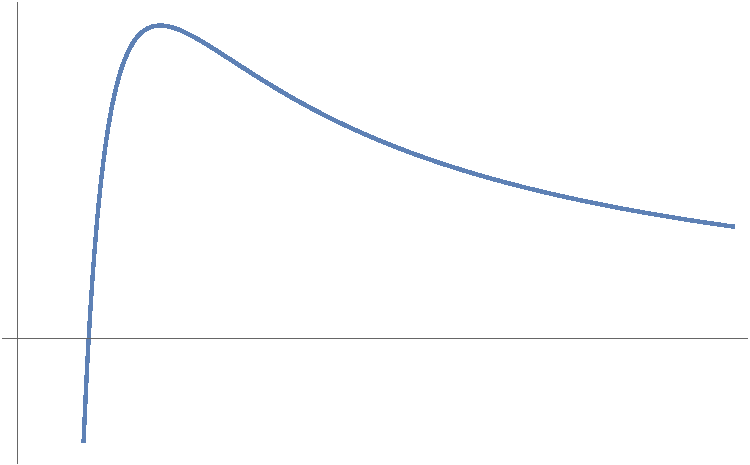
\includegraphics[scale=0.65]{GraficoPV.pdf}
\end{center}

Donde se puede apreciar un punto de máxima presión posible, este es tal que:
$$ \frac{2 a}{v^3} = \frac{R T}{(v-b)^2} $$






\end{document}